\documentclass[AMA,Times2COL]{WileyNJDv5}

\articletype{Perspective}

\received{Date Month Year}
\revised{Date Month Year}
\accepted{Date Month Year}

\journal{Batteries \& Supercaps}
\volume{00}
\copyyear{2026}
\startpage{1}

\raggedbottom

\begin{document}

\title{From Loss Accounting to Feedback Loops: A Coupling Framework for Electrochemical Aging in Lithium-Based Batteries}

\author[1]{Huy Hoang Le}

\author[2]{Kim-Anh Nguyen}

\authormark{LE and NGUYEN}
\titlemark{From Loss Accounting to Feedback Loops}

\address[1]{\orgdiv{R\&D Department}, \orgname{PowerMore Ltd.}, \orgaddress{\city{Da Nang 550000}, \country{Vietnam}}}

\address[2]{\orgdiv{Faculty of Electrical Engineering}, \orgname{University of Science and Technology, The University of Danang}, \orgaddress{\city{Da Nang 550000}, \country{Vietnam}}}

\corres{Corresponding author Kim-Anh Nguyen, Faculty of Electrical Engineering, University of Science and Technology, The University of Danang, Da Nang 550000, Vietnam. \email{nkanh@dut.udn.vn}\\ORCID: Kim-Anh Nguyen 0000-0003-3408-847X; Huy Hoang Le 0009-0009-2138-5468.}

\abstract[Abstract]{Capacity fade in lithium-based batteries is reported mechanism by mechanism: an interphase study quotes Coulombic efficiency, a fracture study crack density, a cathode study parts-per-million dissolved manganese. Each is rigorous, yet the three cannot be combined into one account of why a given cell failed at a stated cycle. The mechanisms are not additive: dissolution and fracture create fresh surface, feeding interphase growth and plating, which raise the overpotential that drives both. Four feedback loops therefore convert linear fade into a sharp knee, and since each closes on a comparison between an accumulated quantity and an available margin, the knee is a design variable. All capacity loss passes through three channels --- loss of lithium inventory (LLI), loss of active material (LAM), kinetic or polarization loss (KL) --- and each mechanism leaves a characteristic trajectory, not a magnitude. Applied to 24 published cells, the prescription returns a positive coupling strength in 22, and the knee moves 2-fold for a 1.3-fold change in the operating margin against a 400-fold change in loop gain. We state six falsifiable predictions, a decision tree that tests whether coupling is present, and a minimum reporting set.}

\keywords{coupling; degradation; feedback loops; knee; lithium-ion batteries}

\maketitle



\begin{table*}[!t]
\begin{center}
\begin{minipage}{\textwidth}
\hrule\vspace{3pt}
\noindent\textbf{Box 1. Terms used in this Perspective.} \textbf{Knee.} The cycle at which fade stops being gradual and becomes abrupt. \textbf{Interphase.} The nanometer film where electrolyte meets electrode, through which lithium must pass. \textbf{Plating.} Lithium deposited as metal instead of entering the anode, which usually shortens life sharply. \textbf{LLI, LAM, KL.} Loss of lithium inventory, of active material, kinetic or polarization loss: the three channels through which capacity disappears. \textbf{C-rate.} How fast a cell is charged or discharged relative to its capacity; 1\,C empties it in one hour. \textbf{Margin.} The gap between a loop's operating value and the threshold where it runs away.
\vspace{3pt}\hrule
\end{minipage}
\end{center}
\end{table*}

\section{Introduction}\label{sec:Introduction}
A cell that has lost 20\% of capacity is described by several mechanisms at once: a thickened interphase,\cite{adenusi2023lithium} a reconstructed cathode surface,\cite{tornheim2019effect} cracked particles.\cite{wheatcroft2023fracture} Each description is defensible and correctly measured. Together they still do not say why this cell reached that loss at that cycle. The gap is compositional, not experimental.

The gap shows as disagreement. Cells of identical chemistry, same materials and process, reach 80\% retention at cycle counts differing by an order of magnitude. Fade is gradual for most of life, then abrupt; the cycle at which it turns is the knee. Were the knee a materials property, identical chemistry would place it identically; it does not.

The mechanisms feed one another: one mechanism's product changes the driving force for another (Figure~\ref{fig1}c), so the set is a dynamical system with thresholds, not a list to sum. Each loop closes when the accumulated quantity overtakes the margin available for it: rate, temperature, voltage window, stack pressure, electrolyte volume, and the anode's own headroom above 0 V. These are set by design and use, not universal constants. The knee is therefore a design variable: that is the claim.

Making the claim usable needs what a catalogue lacks: a unit in which every mechanism counts, and a diagram of which acts on which (Figure 1a). That unit is the capacity channel: loss of lithium inventory (LLI), loss of active material (LAM), or kinetic or polarization loss (KL).\cite{birkl2017degradation,mndezcorbacho2024dest} The diagram runs through surface and overpotential.

Its absence shows as three reporting failures. Fade is quoted without rate, window, temperature, pressure, or format, so nominally identical results are incomparable.\cite{pastorfernndez2019critical} Impedance rise is attributed to interphase growth without separating it from other sources, making the attribution unfalsifiable.\cite{edge2021lithium} The knee is fitted, not derived.\cite{diao2019algorithm} Each reports a quantity without its margin.

The claim is testable: it predicts which operating variable moves the knee in a given cell (Table~\ref{tab2}) and supplies a decision tree separating the loops (\S6). A knee that fails to move under all four perturbations is evidence against coupling.

Prior work stops at the catalogue. Attia et al. classify knee trajectories, and their "snowball" class is the loop described here in earlier vocabulary, but they treat the knee as a feature to detect, not the output of a coupled system.\cite{attia2022review} Yu, Zhu and Yu consolidate the cathode-side cascade and close with mitigation, a cathode-limited structure that cannot count inventory the anode destroys.\cite{yu2026degradation} What we add is the accounting unit and the failure criterion: inventory across the whole cell, and predictions stating what would refute them.\cite{raj2020investigation}

One last observation sets the scale. For every loop the ratio of operating value to threshold falls within two orders of magnitude, ratios of roughly 1 to 100 (SI S2), so no loop is negligible. Cell design has co-optimized several degradation thresholds, placing well-designed cells closest to several margins and making them especially susceptible to coupling-induced knees.




\begin{figure*}[t]
\centerline{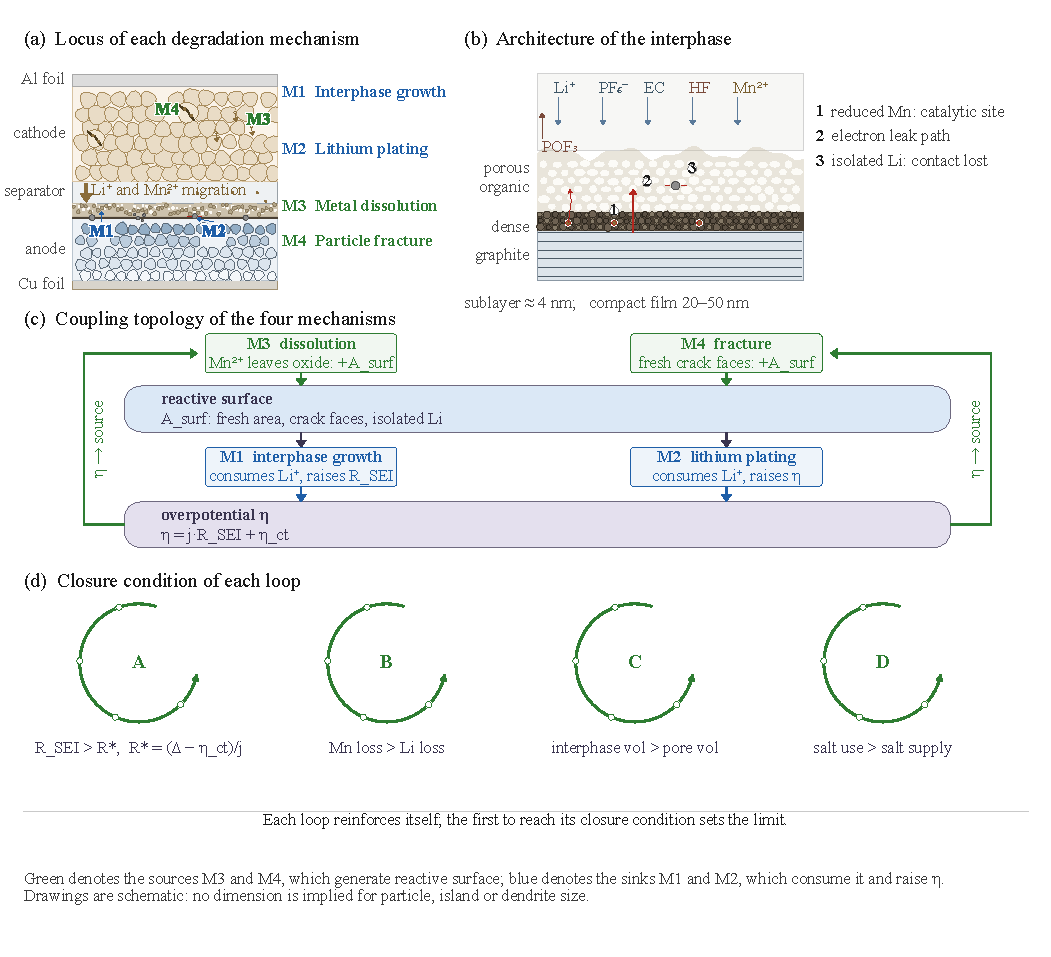
\includegraphics[width=\textwidth]{figure-mechanism}}
\caption{Four mechanisms, two state variables, four limiting conditions. Mechanism drawing: no computed curve, no lifetime. \textbf{(a)} Locus of each mechanism in a cell section. Dissolution (M3) and fracture (M4) generate reactive surface; interphase growth (M1) and plating (M2) consume lithium inventory and surface. \textbf{(b)} Interphase architecture: a dense inorganic sublayer of a few nanometers under a porous organic region of tens of nanometers, leaky, not blocking, so a film thicker than the tunneling limit keeps growing until the pore volume fills. \textbf{(c)} Sources feed one surface rail and sinks one overpotential rail, reducing four mechanisms to two. \textbf{(d)} Engagement condition of each loop: the gap in each circle is the inequality under which the loop runs away. It marks onset, not termination. Schematic: no scale implied.}
\label{fig1}
\end{figure*}

\section{Loss accounting and the trajectory}\label{sec:Lossaccountingandthetrajectory}
Capacity is lost through three channels. LLI is lithium that can no longer be cycled: bound in the solid--electrolyte interphase (SEI), trapped in electrically isolated metal, or sequestered in closed porosity. LAM is host that can no longer store lithium: fractured or disconnected particles, phase-transformed material, delaminated composite. KL is capacity that exists thermodynamically but is inaccessible at the applied rate. Each is defined by what is gone, not by the measurement that detects it.\cite{birkl2017degradation}

The decomposition is complete for capacity: lithium not cycled is present but inaccessible at this rate (KL) or converted to a non-cyclable form (LLI), and an active site either functions or not (LAM). LLI and KL are not orthogonal at finite rate, so a reference rate and temperature must be quoted (\S8).

The decomposition is standard and automated,\cite{mndezcorbacho2024dest} and the modes are extracted by fitting open-circuit-voltage curves.\cite{dubarry2012synthesize} The claim here is narrower: trajectories are diagnostic. Each mechanism moves the channels in a characteristic order and time law, and that ordering discriminates where magnitude cannot. A cathode losing active material moves LAM before LLI; a plating-limited anode moves LLI while LAM stays flat; a cell whose impedance has grown moves KL with little capacity change. Magnitudes reflect history and do not transfer between cells; orderings reflect mechanism and do.

The practical consequence changes what is fitted. With $f = 1 - \mathrm{CE}$ (Coulombic efficiency), retention obeys $Q(N)/Q_0 = 1 - fN$, so $N_R = (1 - R)/f$. This is straight only if \emph{f} is constant, so downward curvature measures $\mathrm{d}f/\mathrm{d}N$, the coupling strength. A fitted slope returns an average CE and conceals loop closure;\cite{smith2010precision} fit $f(N) = f_0 + \alpha N$ and report $\alpha$ with its window; no new experiment is required.

One limitation applies. The decomposition is complete for capacity, not energy: voltage fade in Mn-rich and Li-rich oxides is a thermodynamic shift of the host potential, decoupled experimentally from capacity fade.\cite{pang2025resolving} Reporting energy fade would need a fourth channel, which we name an open problem.


\begin{table*}[t]
\caption{First channel to move, and time law, for each mechanism. The ordering discriminates; the magnitude does not.}
\label{tab1}
\begin{tabular*}{\textwidth}{@{\extracolsep\fill}lll@{}}
\toprule
Mechanism & First channel to move & Time law\\
\midrule
M1 interphase growth & LLI & steady accumulation; anode impedance grows while LAM stays flat\\
M2 lithium plating & LLI & accelerating; voltage hysteresis grows\\
M3 metal dissolution & LAM and LLI together & the two rise in step; Mn detected on the anode\\
M4 particle fracture & LAM, then LLI & stepwise; responds to stack pressure, not to the voltage window\\
\bottomrule
\end{tabular*}
\end{table*}

\section{Sources and sinks}\label{sec:Sourcesandsinks}
The four mechanisms of Figure 1a are not equivalent. Dissolution (M3) and fracture (M4) act as sources: they generate reactive surface, enlarging the area for parasitic reaction.\cite{single2018identifying} Interphase growth (M1) and plating (M2) act as sinks: they consume lithium inventory and electrolyte (Figure 1b).\cite{nojabaee2021understanding,brown2021detecting} Sources set gain and sinks the offset. The classification is imperfect: dead lithium is a sink that also adds surface, and we retain that hybrid.

Independence has an exact operational meaning, and it fails. Were the four mechanisms independent, the loss with all four running would equal the sum measured one at a time. It does not: a cathode releasing manganese shortens the life of an anode it never touches, and a crack consumes inventory the fracture did not remove.\cite{santos2023chemistry} Independence is falsifiable and already refuted.

A loop exists only if one mechanism's product is another's input, and only two quantities pass that way: fresh reactive surface, created by dissolution and fracture and consumed by interphase growth and plating, and local overpotential, raised by the sinks and exploited by the sources. The four mechanisms therefore reduce to two state variables, and all four loops run between them (Figure~\ref{fig1}c).

The relation between sources and sinks carries more information than any arrow, because sources are not conserved. A little dissolution can be amplified into substantial inventory loss; a little interphase is unlikely to become substantial fracture. That gain asymmetry is a prediction: a cell with only sinks degrades monotonically, since a sink lowers the fade intercept while only a source raises its slope. The margin is the distance from a loop's operating value to the threshold at which it self-sustains, and design sets that distance.

\section{The four loops}\label{sec:Thefourloops}
Each loop has four elements, each with an evidence grade: driving force, pathway, observable, and engagement condition. Well supported: mechanism measured, feedback observed in relevant cells. Supported: mechanism measured, feedback inferred. Mechanism supported, feedback untested: ingredients measured, interaction not.

\textbf{Loop A. Plating $\rightarrow$ dead lithium $\rightarrow$ more interphase $\rightarrow$ higher local overpotential $\rightarrow$ more plating.} The driving force is the local anode potential falling below 0 V vs Li/Li$^{+}$. Lithium reduced at the graphite-separator interface is partly isolated on stripping, and the dead metal carries fresh interphase that raises local impedance and pushes the next charge below 0 V.\cite{hsieh2020quantification,vil2020nickel,betz2019cross} The observable is superlinear inventory loss with rising hysteresis and an efficiency decline cathode impedance cannot explain. The loop closes when $R_{\mathrm{SEI}} > R^{\ast} \equiv (\Delta-\eta_{\mathrm{ct}})/j$, where $\Delta$ is the margin between the operating anode potential and 0 V, $\eta_{\mathrm{ct}}$ the charge-transfer overpotential, and $j$ the local current density. $R^{\ast}$ is a ratio of operating quantities, not a fixed number. Evidence grade: well supported.

\textbf{Loop B. Dissolution $\rightarrow$ anode poisoning $\rightarrow$ interphase destabilization $\rightarrow$ more inventory loss.} The driving force is thermodynamic instability of the cathode surface: Mn$^{3+}$ disproportionation, HF attack from salt hydrolysis, oxygen loss at high voltage.\cite{tesfamhret2023role,sharifiasl2019oxygen,huang2021understanding} Dissolved cations cross the separator, are reduced at the anode, and enter the interphase, while the cathode surface reconstructs to rock salt. The observations move together: oxygen loss, reconstruction-layer growth, rising interfacial impedance, and transition-metal loading on the anode.\cite{tornheim2026quantifying,gilbert2017transition} That correlated quartet discriminates, since no single-mechanism account predicts all four. Acid generation is autocatalytic and potential-gated, which closes the loop. Dissolution is not stoichiometrically sufficient. At an assumed 5 ppm of the cathode's manganese inventory per cycle, 0.5\% leaves over 1000 cycles; even if each departing Mn$^{2+}$ destroyed one Li$^{+}$, that removes 0.27\% of the lithium inventory against a $\sim$20\% capacity loss --- a 74-fold shortfall --- so the damage must be catalytic. One estimate puts it at $\sim 10^{2}$ trapped Li$^{+}$ per deposited Mn ion, the order the arithmetic needs, though it is an estimate whose Mn-free control also changes Ni and Co, and it remains unverified.\cite{woodford2010electrochemical} Evidence grade: supported.

\textbf{Loop C. Fracture $\rightarrow$ fresh surface $\rightarrow$ interphase growth $\rightarrow$ local stress $\rightarrow$ more fracture.} The driving force is diffusion-induced stress, $\nabla c \rightarrow \nabla\sigma$, amplified by second-phase stiffness mismatch.\cite{pandurangi2023chemo,deshpande2017modeling} Cracking exposes unpassivated surface that consumes lithium at once; the interphase then fills pore volume, becomes load-bearing, and changes the particle's constraint.\cite{ai2022coupled,carelli2022coupling} Gradient stress is rate-dependent and fades at slow cycling, so a low-rate sweep appears to exonerate fracture; coherency stress is rate-independent and survives any C-rate. A sweep probes only the first, so a null result at low rate does not test the loop. The observable is active-material loss leading inventory loss, sensitive to stack pressure not voltage window. It closes when interphase-filled pore volume sets the fracture threshold: 1 mAh\,cm$^{-2}$ of inventory loss makes ~11 \textmu m of dense interphase-equivalent volume, so a 10 \textmu m, 30\%-porosity coating fills after 0.3--0.6 mAh\,cm$^{-2}$ (10--20\% of capacity), while the ~77 \textmu m anode matched to a 3 mAh\,cm$^{-2}$ cathode fills only after ~2 mAh\,cm$^{-2}$ (68\%). Loop C closes early on thin anodes, late on conventional ones. Evidence grade: mechanism supported, timing loading-dependent.

\textbf{Loop D. Electrolyte depletion $\rightarrow$ transport limitation $\rightarrow$ higher local overpotential $\rightarrow$ more plating and more interphase.} The driving force is consumption of salt and solvent by the accelerated reactions, plus transference-number polarization.\cite{lithiummetal2026science,fang2019quantifying} Transport limitation concentrates current on the electrode nearest the separator; fade scales with thickness, not chemistry. The loop closes when salt consumption outruns diffusion: a lean cell at 1 g\,Ah$^{-1}$ holds $\sim$3.3 $\mathrm{\mu mol\,cm^{-2}}$ of salt against the $\sim$30 $\mathrm{\mu mol\,cm^{-2}}$ that 0.8 mAh\,cm$^{-2}$ of inventory loss consumes, an 8.95-fold exceedance. Evidence grade: mechanism supported; feedback untested.

Two loops carry a caveat. Loop A counts its sink as interphase-bound lithium, but titration gas chromatography counts unreacted Li$^{0}$ as H$_2$; interphase-bound Li$^{+}$ does not react with that reagent.\cite{smith2010precision} In lithium-metal cells unreacted Li$^{0}$, not interphase-bound Li$^{+}$, dominates the inactive lithium, so the field may have mis-partitioned, not mismeasured. Loop B's gain is the open question. The effect is not in doubt: manganese in solution raises parasitic current at graphite.\cite{dubarry2012synthesize} Missing is a scaling law for the magnitude, without which no account can say what the loop does to the trajectory. It is decidable: if spiking reproduces under 10\% of the observed fade, the loop is unnecessary and the arrow points to cathode impedance instead.

\section{The knee as a design variable}\label{sec:Thekneeasadesignvariable}
A knee is a change in the composition of loss, not merely in slope: the marginal loss shifts toward inventory loss, or the inventory exponent exceeds 1. It is testable on any decomposed curve.

No rate law is discontinuous. Each mechanism's rate is smooth in its own arguments, so a knee requires a system property: gains below a threshold restore the operating point after a perturbation, gains above it do not. Smooth laws therefore give a sharp transition, and a single-exponential fit succeeds locally but fails to predict. Which loop reaches the boundary first is set by operating conditions: high rate and low temperature select Loop A, high voltage and a manganese-rich cathode Loop B, high stack pressure Loop C, thick electrodes and lean electrolyte Loop D. Only Loop A is modeled here, so the assignment for B, C and D is an argument from the mechanism, not a result (SI S1.10). This accounts for identical chemistry showing different fade and for a cycle life quoted without these parameters being unphysical (Figure~\ref{fig1}d). Such a transition is published for plating on graphite.\cite{klein2024identifying}

A controlled contrast tests it. In a reduced Loop A model (SI), zeroing the feed-forward gain delays the knee from 530 to 670 cycles and capacity loss from 1044 to 1681; zeroing the dead-lithium fraction abolishes it within 6,000 cycles. The response is inelastic: a 400-fold gain change moves the knee about 2.2-fold, as a threshold crossing predicts, since gain sets how fast the margin is consumed, not where the boundary lies. Sweeping the margin separates the two: over a 1.33-fold window, chosen so plating starts after the departure detector's baseline, the knee moves 2.14-fold, so a 300-fold larger gain change buys about the same shift (SI S1.16). The severings are not equivalent: the dead-lithium fraction also removes an inventory sink, so the arrow is not isolated. It holds at 0.5 and 1 C, not 2.0 C. One limit qualifies it: the most influential margin is the least controllable, being set by the anode equilibrium potential, not a process setting.

Two evidence forms answer different questions: the margin sweep tests the mechanism; what follows asks only whether the quantity \S2 asks for, $\alpha$, is obtainable from published data. Harris et al. cycled 24 commercial pouch cells at 10 C and reported retention per cycle.\cite{harris2017failure} Fitting $f(N) = f_0 + \alpha N$ over 100\% to 90\% retention gives $\alpha > 0$ in 22 of 24 cells, median $5.6\times10^{-7}$ per cycle. A constant \emph{f} leaves 0.042 RMS in retention, a quadratic 0.008 with negative curvature in all 24; three independent estimates agree (SI S1.15). The limit is as plain: over 95--100\% retention $\alpha > 0$ in only 6 of 24, since early-cycle noise exceeds the curvature, so $\alpha$ is window-dependent and incomparable across studies that do not fix it. Positive $\alpha$ shows efficiency loss accelerates; it does not say which channel, since retention alone cannot separate LLI from LAM.

The model also fails a test the framework ought to pass. If the knee is an early-warning object, life must remain after it, and the model's knee-to-life ratio does not discriminate against published cells (SI S1.13). Its knee is its end of life under the manuscript's convention, a ratio of 1.00 against a published median of 1.26, with alternative conventions spanning 1.00--1.91. A test whose outcome is set by its own definition has no discriminating power, so we report it as inconclusive. What survives is weaker: fade accelerates after the knee in 13 of 19 cells (SI S1.14). The claim rests on operating-variable dependence, not on this ratio.

\section{Diagnostic separability}\label{sec:Diagnosticseparability}
Separability makes the predictions of \S7 testable. The decision tree in SI S4 organizes diagnostics by loop, because a loop leaves a curvature signature in time that a mechanism does not, and each branch ends in a failing test.\cite{prosser2021lithium,costa2022battery,gunnarsdottir2020noninvasive} SI Table S1 indexes each measurement; three confounds remain: interphase-bound and metallic lithium cannot be separated by coulometry alone, since both consume electrons without intercalation;\cite{mcshane2020quantification} fracture-driven and reconstruction-driven loss both register as inactive material, needing post-mortem imaging; and electrolyte depletion and contact loss give superimposable impedance spectra. That last gap is the most restrictive.

\section{Six falsifiable predictions}\label{sec:Sixfalsifiablepredictions}

\begin{table*}[t]
\caption{Predictions, loops tested, refutation conditions, and data status.}
\label{tab2}
\small
\begin{tabularx}{\textwidth}{@{}l>{\raggedright\arraybackslash}X>{\raggedright\arraybackslash}X>{\raggedright\arraybackslash}p{0.17\textwidth}@{}}
\toprule
 & Prediction & Refuted if & Data status\\
\midrule
P1 (Loop C) & Identical chemistry at different stack pressure shows knees at different cycle counts & the knees coincide & already published\\
P2 (Loop A) & Anode-free and graphite cells at matched inventory-loss rate show different efficiency curvature & the curvatures coincide & new experiment\\
P3 (Loop B) & Suppressing dissolution moves the slope of inventory loss, not its intercept & only the intercept moves & re-analysis\\
P4 (Loop D) & At fixed total additive mass, electrolyte loading in g~Ah$^{-1}$ predicts life & life is invariant & re-analysis\\
P5 (Loop C) & Single-crystal and polycrystalline material differ in knee sharpness, not initial fade rate & fade rates differ while knee shape does not & already published\\
P6 (all loops) & Retention is concave over a pre-registered window no narrower than 90\% & a majority of cells are convex over that window & checked here (SI S1.15)\\
\bottomrule
\end{tabularx}
\end{table*}

Each prediction names a contrast and what would refute it (Table~\ref{tab2}).

\textbf{P1:} identical chemistry at different stack pressure shows knees at different cycle counts; refuted if they coincide.\cite{wang2026interplay,barai2017effect} \textbf{P2:} anode-free and graphite cells at matched inventory-loss rate show different efficiency curvature, since only the metal system closes Loop A; refuted if they coincide.\cite{louli2019exploring} \textbf{P3:} suppressing dissolution moves the \emph{slope} of inventory loss, not its intercept; refuted if only the intercept moves. \textbf{P4:} at fixed total additive mass, electrolyte loading in g\,Ah$^{-1}$ predicts life; refuted if life is invariant. The qualifier matters: added electrolyte carries added additive inventory, and irreversible loss grows with electrolyte volume until additive mass is fixed, a confound that could reverse the sign of P4.\cite{lechtenfeld2024electrolyte} \textbf{P5:} single-crystal and polycrystalline material differ in knee sharpness, not initial fade rate; refuted if fade rates differ while knee shape does not.\cite{wheatcroft2024situ} P5 tests only the gradient-stress branch. \textbf{P6:} within a retention window fixed before fitting and no narrower than 90\%, retention is concave in cycle number, which is $\alpha > 0$ in \S2; refuted if a majority of cells are convex over that same window. P6 is the only one testable on data in hand, and \S5 reports such a test (SI S1.15). The window clause is not decoration: over 95--100\% retention the majority is convex, so the window belongs in the prediction or the test is only adjustable.

P3 needs one clarification, since the measurement already exists. Protocols that titrate dissolved transition metal into graphite measure the parasitic current during potentiostatic holds,\cite{meunier2022electrochemical} and they show the amplification occurs. P3 asserts something stricter: that the amplification bends the \emph{slope of the inventory trajectory during cycling}, not only the height of a hold current. A cell can show both and still fail P3.

An unexecutable prediction is not falsifiable. A single mechanism gives monotone fade, a loop gives acceleration, so the inflection in $\mathrm{d}(\Delta Q)/\mathrm{d}N$ locates the onset; perturb one loop-specific variable (temperature for A, an HF scavenger for B, stack pressure for C, electrolyte volume for D) and ask whether the knee moves.\cite{wang2026interplay,louli2019exploring} An insensitive knee is a counterexample, not a null result.

\section{Outlook}\label{sec:Outlook}
A reporting set is one result that transfers; the checklist is in SI S3.4. Among its twenty items, the nine of Tier 1 are load-bearing: loadings, N/P, electrolyte mass, water and HF, format and stack pressure, voltage window, C-rate, temperature, protocol, fade-quoting cycle and trajectory, and formation.\cite{dechent2021estimation} None needs new science; most are already measured. The failure is selective reporting, since a reader cannot reconstruct the margin the cell ran against. A mandatory table would make the corpus comparable and allow retrospective loop testing.

The least demanding test is spiking: introduce dissolved transition metal at the flux inferred in \S4 and ask whether the parasitic current rises as predicted. The others need local anode-potential mapping, isotope-resolved metal flux, crack-resolved operando tomography, and salt-concentration imaging, all of which exist but none routinely.

Two problems remain open. No non-destructive method partitions metallic from interphase-bound lithium in a sealed cell, and energy fade has no accepted channel. A demonstration that life is invariant to electrolyte loading would remove Loop D and leave three.

Within these limits, failure at a given cycle is a sequence of loop closures, and a design outcome.

\bmsection*{Conflict of interest}
The authors declare no conflict of interest.

\bmsection*{Data availability statement}
This Perspective reports no new experimental data. The derivations that underpin every number quoted in the text, and the Supporting Information display items, are provided as Supporting Information. The reduced model is specified in Section S1 of the Supporting Information in sufficient detail to be re-implemented from the stated equations and parameters.

\bmsection*{Acknowledgements and funding}
This work received no specific funding from any agency in the public, commercial, or not-for-profit sectors.

\bibliography{references}

\end{document}
